\chapter{Design}
\label{chap:design}

\section{System Sequence Diagram}
\label{sec:system_sequence_diagramm}
Die System Sequence Diagramme zeigen die möglichen Interaktionen 
von extern mit unserem Mindmap Programm.

\begin{figure}[H]
	\centering
		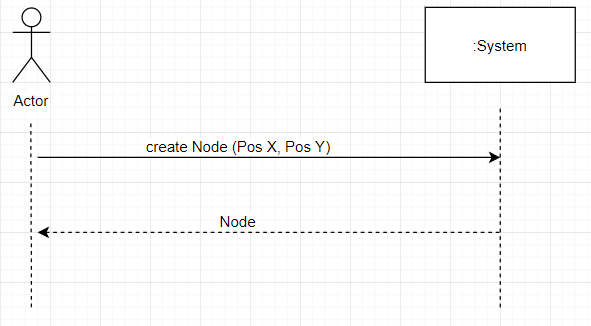
\includegraphics[scale=0.7]{images/createnode.PNG}
	\caption{Create Node SSD}
	\label{fig:create_node_ssd}
\end{figure}

Der Benutzer übergibt dem System eine Position in welcher er den Node erstellen möchte, das System
erstellt dann den Node mit allen seinen Komponenten, also der Form, dem Text und den Anchors für das
Verbinden.

\begin{figure}[H]
	\centering
		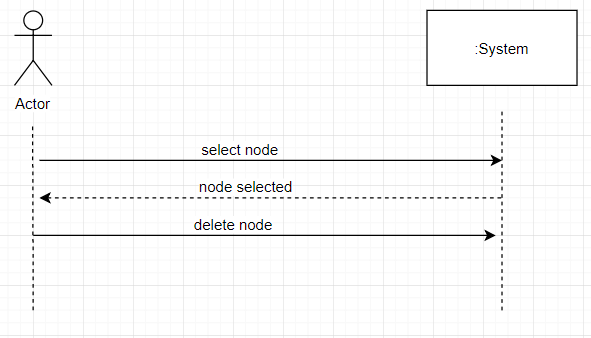
\includegraphics[scale=0.7]{images/deletenode.PNG}
	\caption{Delete Node SSD}
	\label{fig:delete_node_ssd}
\end{figure}
Der Benutzer wählt einen Node oder eine Verbindung(der Ablauf zum Löschen eines Nodes oder einer Verbindung ist gleich), das System löscht diesen Node dann vom GUI und von der Liste. 

\begin{figure}[H]
	\centering
		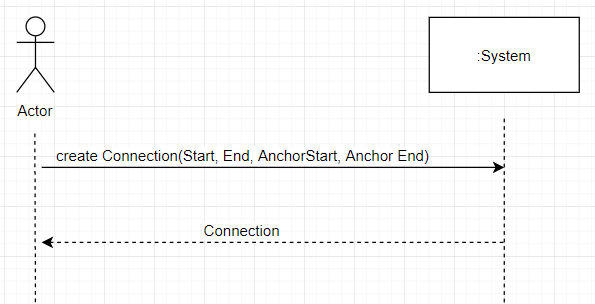
\includegraphics[scale=0.7]{images/createconnection.PNG}
	\caption{Create Connection SSD}
	\label{fig:create_connection_ssd}
\end{figure}
Der Benutzer wählt einen Start und einen Ziel Anchor für seine Verbindung aus, das System erstellt
dann anhand dieser Informationen die Verbindung.

\begin{figure}[H]
	\centering
		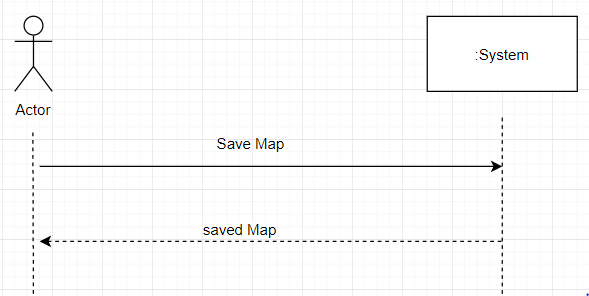
\includegraphics[scale=0.7]{images/savemap.PNG}
	\caption{Save Map SSD}
	\label{fig:save_map_ssd}
\end{figure}
Der Benutzer speichert die Map, das System speichert nun alle Informationen der Map in eine
Datei und übergibt sie dem Benutzer.

\begin{figure}[H]
	\centering
		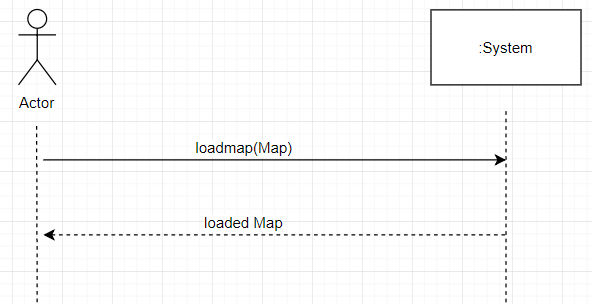
\includegraphics[scale=0.7]{images/loadmap.PNG}
	\caption{Load Map SSD}
	\label{fig:load_map_ssd}
\end{figure}
Der Benutzer lädt eine alte Map und übergibt dem System eine Datei mit den Informationen, das System
arbeitet nun die Informationen ab und stellt die Map dar.

\section{Sequence Diagram}
\label{sec:sequence_diagram}
Das Sequence Diagramm zeigt die Interaktion zwischen den verschiedenen Objekten in dem Mindmap System.
\begin{figure}[H]
	\centering
		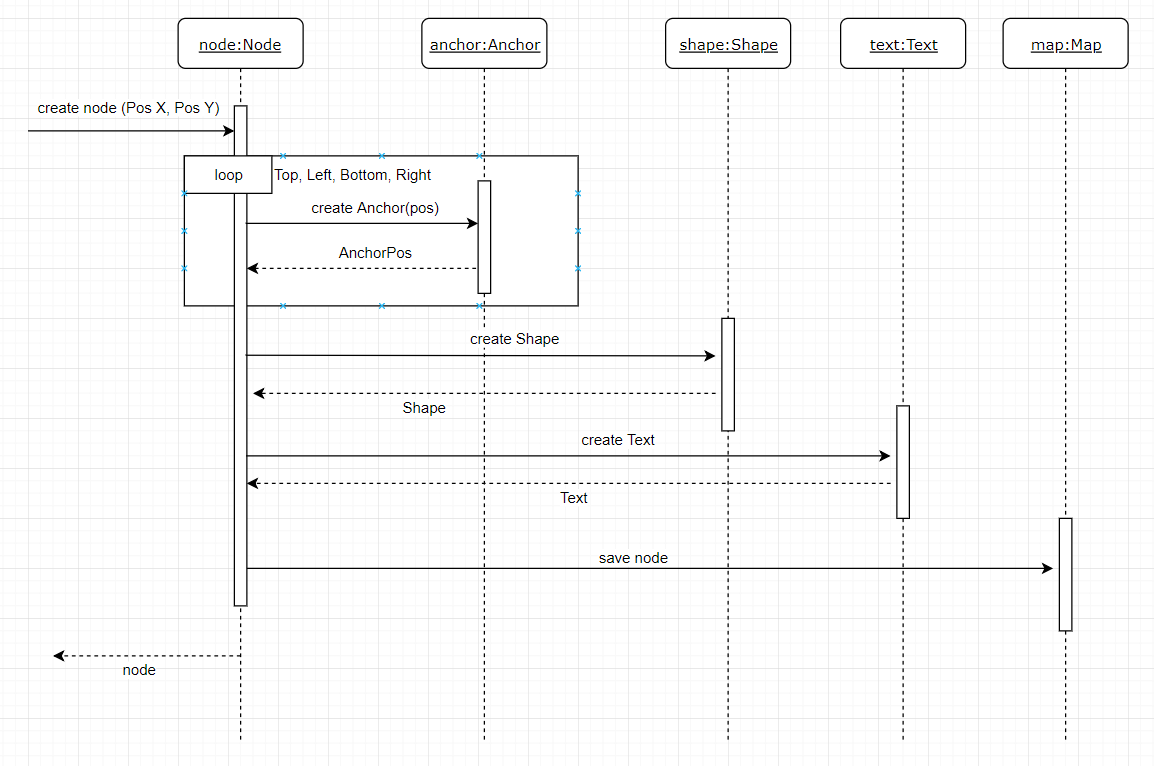
\includegraphics[width=\textwidth]{images/crNodeSD.PNG}
	\caption{Create Node SD}
	\label{fig:create_node_SD}
\end{figure}

Das System erstellt einen neuen Node, der Node erstellt dann seine Objekte welche er benötigt.
Er erstellt ein Shape für seine Form, er erstellt einen Text für die Beschreibung und er erstellt
4 Anchors(TOP,LEFT,BOTTOM,RIGHT) für das Verbinden der Knoten. Danach wird der Knoten in die Maplist 
gespeichert.

\begin{figure}[H]
	\centering
		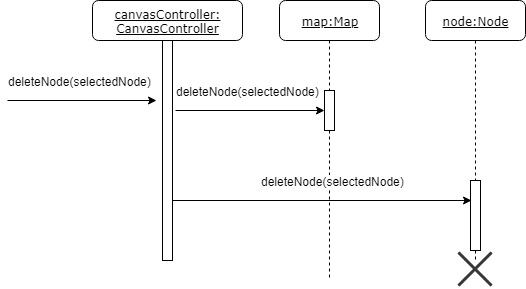
\includegraphics[scale=0.6]{images/delNodeSD.PNG}
	\caption{Delete Node SD}
	\label{fig:delete_node_SD}
\end{figure}

Das System löscht den selektieren Knoten von der Map und löscht diesen dann von der Liste. 
Dies funktioniert gleich bei der Verbindung.

\begin{figure}[H]
	\centering
		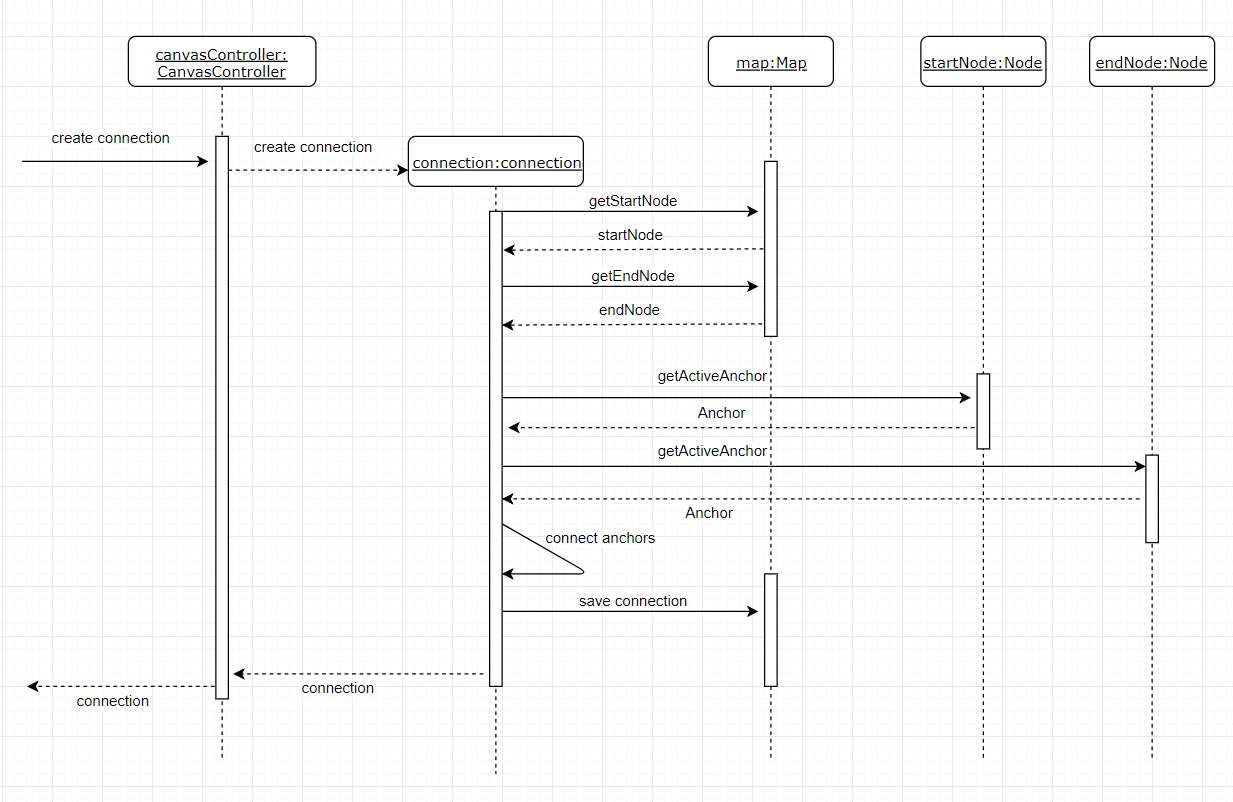
\includegraphics[width=\textwidth]{images/connectionSD.PNG}
	\caption{Create Connection SD}
	\label{fig:create_connection_SD}
\end{figure}
Das System erstellt eine neue Verbindung, es holt sich zuerst die beiden aktiven Knoten, den Start 
und den End Knoten. Von diesen beiden Knoten holt es sich dann die jeweiligen aktiven Anchors. Danach
verbindet das System die beiden aktiven Anchors miteinander.

\begin{figure}[H]
	\centering
		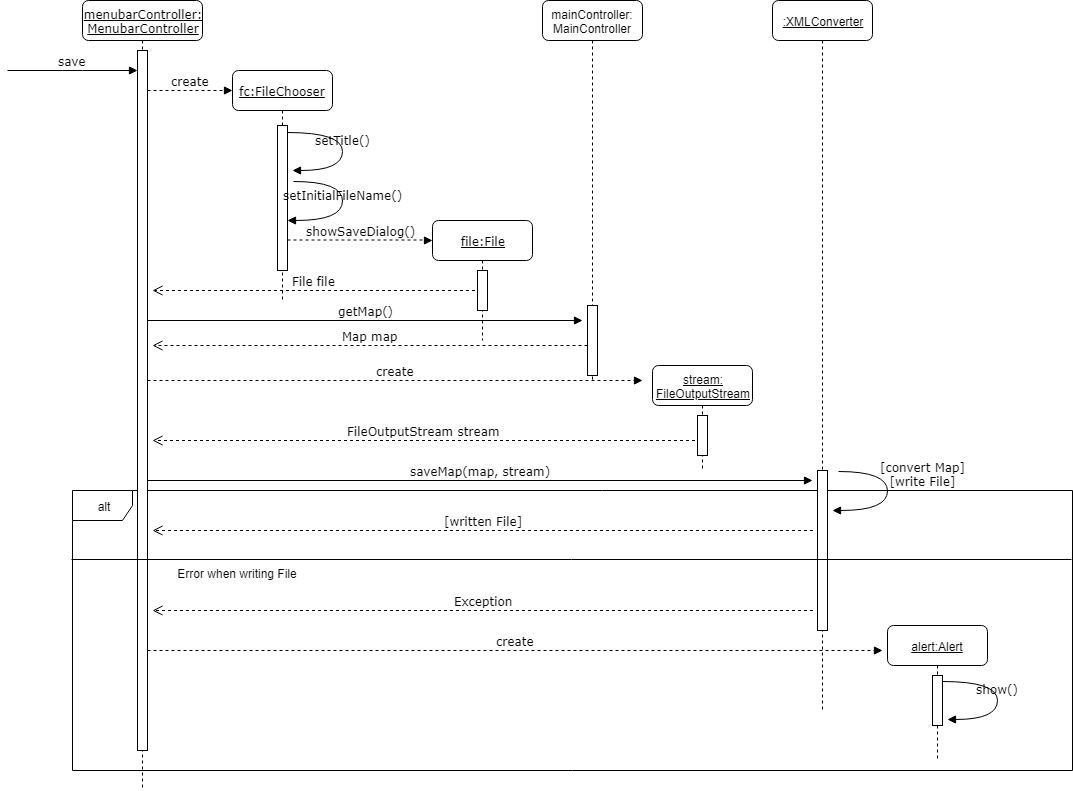
\includegraphics[width=\textwidth]{images/savemapSD.png}
	\caption{Save Map SD}
	\label{fig:savemap_SD}
\end{figure}
Das System lässt den Benutzer eine Datei wählen und erzeugt einen OutputStream. Die Map des MainControllers und der Stream werden dem XMLConverter übergeben. Dieser konvertiert die Map in ein speicherbares Objekt und schreibt die XML Datei. Die Funktionalität des XMLConverters ist im nächsten Sequence Diagram ersichtlich.

\begin{figure}[H]
	\centering
		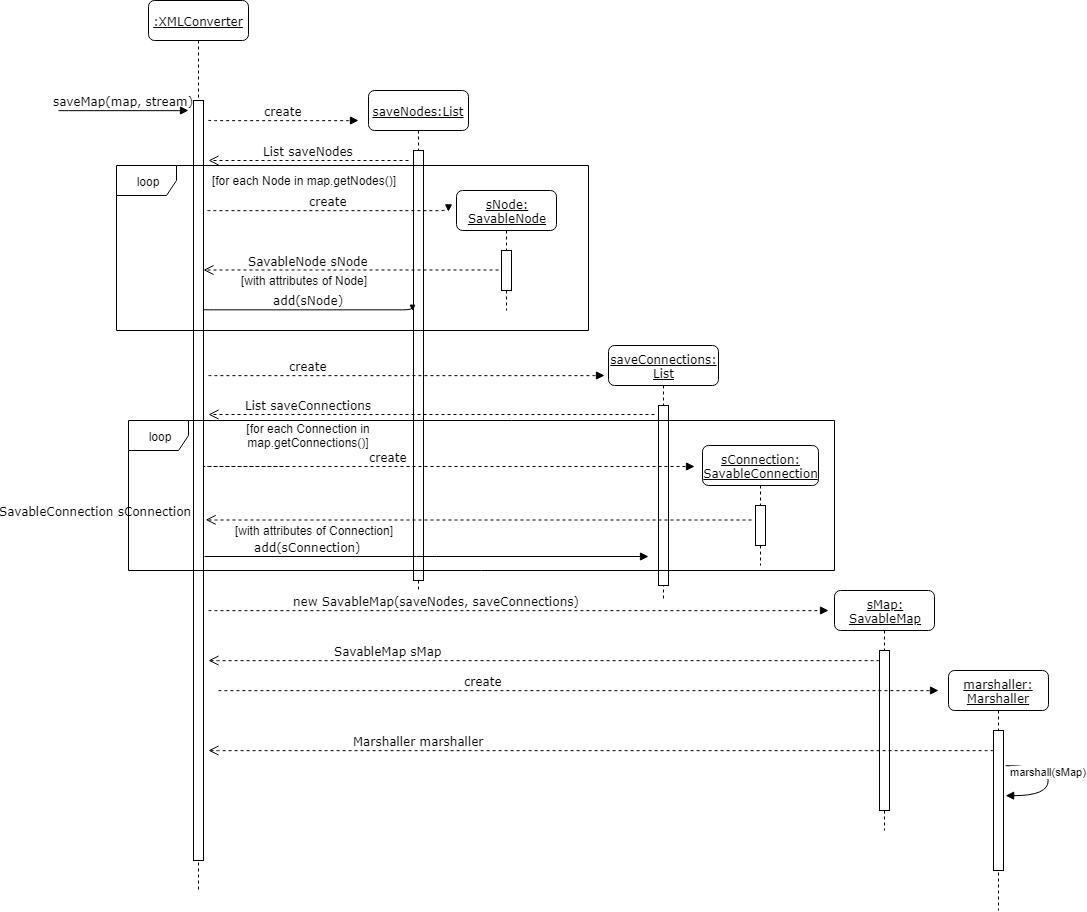
\includegraphics[width=\textwidth]{images/saveConvertSD.png}
	\caption{Convert \& Save Map SD}
	\label{fig:saveConvert_SD}
\end{figure}

\begin{figure}[H]
	\centering
		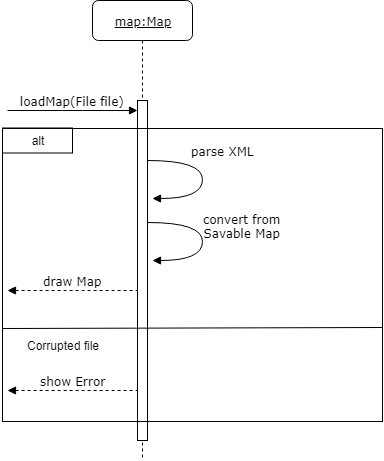
\includegraphics[width=\textwidth]{images/loadmapSD.png}
	\caption{Load Map SD}
	\label{fig:loadmap_SD}
\end{figure}
Das System lässt den Benutzer eine Datei wählen. Der XMLConverter liest die Datei und erzeugt daraus eine Map. Diese wird danach angezeigt.

\begin{figure}[H]
	\centering
		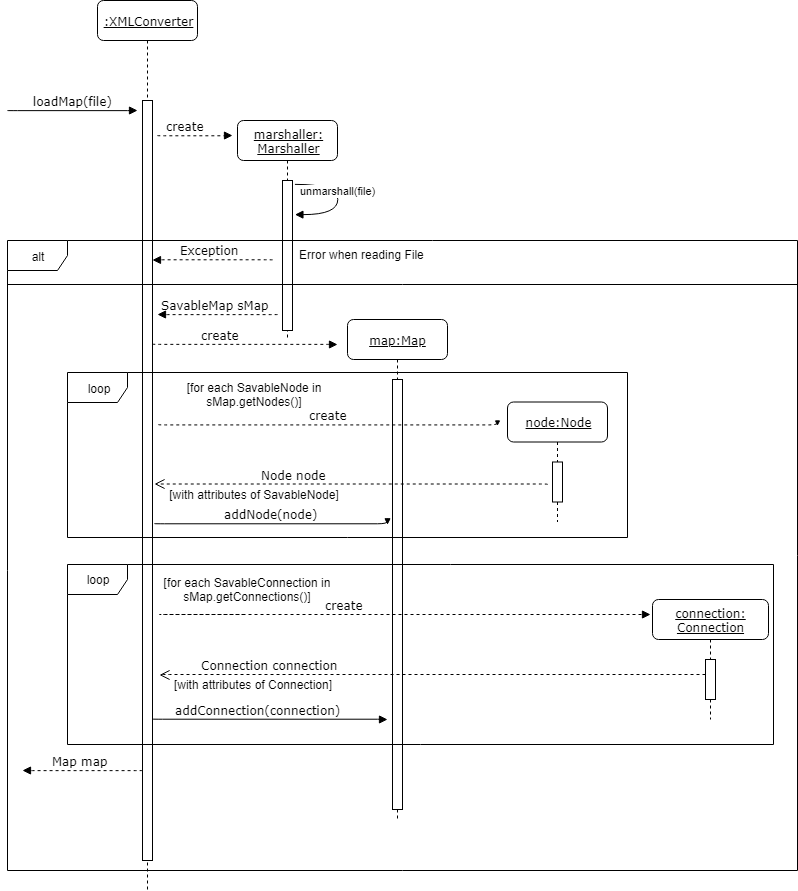
\includegraphics[width=\textwidth]{images/loadConvertSD.png}
	\caption{Load \& Convert Map SD}
	\label{fig:loadConvert_SD}
\end{figure}

\section{Package Diagramm}
\label{sec:package_diagramm}
Unsere Packetstruktur ist nach dem MVC Prinzip erstellt. Wir haben ein View Packet mit den FXML Dateien und dem Main Programm, ein Controller Packet mit den Controllern, ein Util Packet mit den Zusatzfunktionen wie Speichern, Laden und Ordnen und ein Model Packet mit den Objekten wie Node, Connection usw.

\begin{figure}[H]
	\centering
		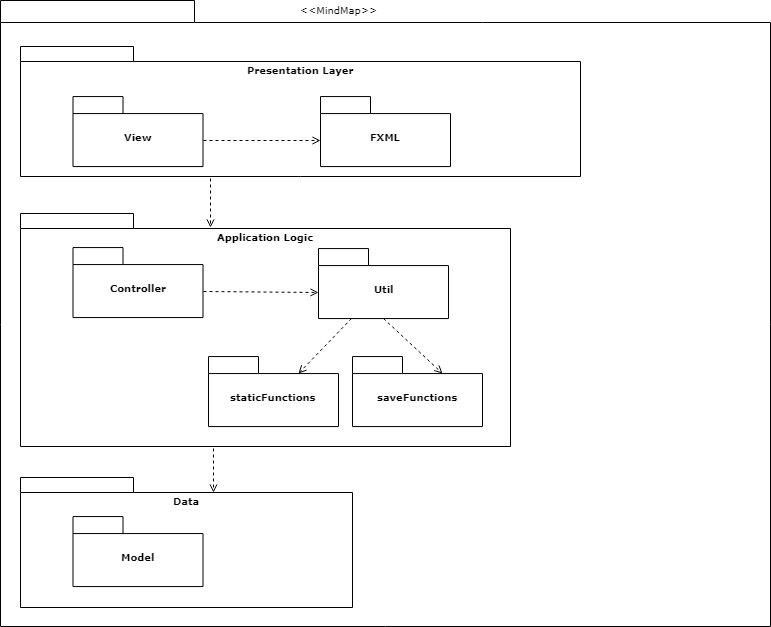
\includegraphics[width=\textwidth]{images/packagediagramm.png}
	\caption{Package Diagramm}
	\label{fig:loadConvert_SD}
\end{figure}


\section{UML Diagramme}
\label{sec:uml_diagramme}

\subsection{Klassen Diagram}
\label{subsec:class_diagramm}
\begin{figure}[H]
	\centering
		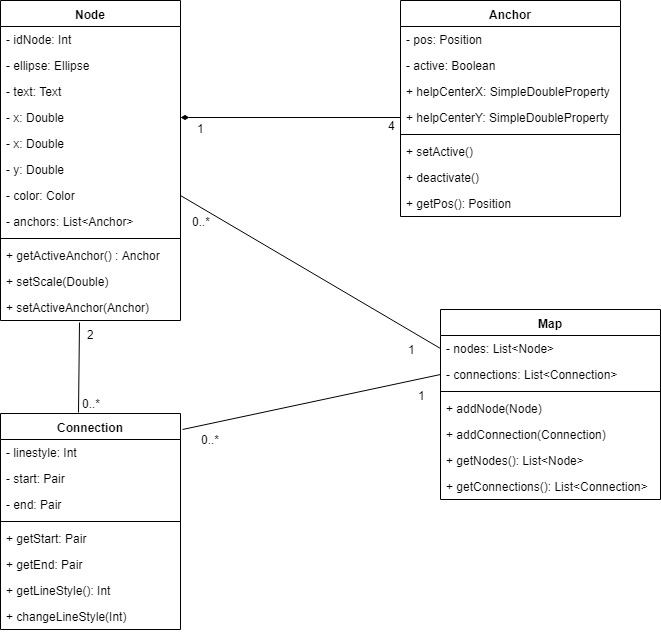
\includegraphics[scale=0.5]{images/class_diagramm.png}
	\caption{Klassen Diagramm}
	\label{fig:class_diagramm}
\end{figure}

Das Klassen Diagramm zeigt einige der wichtigen Klassen in unserem Programm, deren Eigenschaften und wichtige Funktionen.
\begin{itemize}
\item \textbf{Map}: Eine Map hat eine Liste von Nodes und eine Liste von Connections. Entsprechend können diese ausgelesen oder neue Einträge in den Listen gemacht werden.
\item \textbf{Node}: Eine Node enthält die vom Programm gezeigte Ellipse und die dazugehörige Position sowie den Text.
\item \textbf{Connection}: Eine Connection verbindet zwei Nodes (Start und Ende) als Linie.
\item \textbf{Anchor}: Eine Node hat 4 Anchors an denen eine Linie beginnen kann.
\end{itemize}